\section{Cabo de Comunicação}
\label{cabo_01}


\begin{table}[ht!]

	\begin{tabular}{r l|l p{12cm} }
		
		\textcolor{gray}{Especificação} &&& 	{Cabo de Comunicação}\\
		\textcolor{gray}{Data} &&& 				{10/02/2015}\\
        \textcolor{gray}{Beneficiado} &&&		{Cabos Lapp Brasil}\\
        \textcolor{gray}{CNPJ} &&& 				{05.233.912/0001-27}\\
        \textcolor{gray}{Número Nota} &&& 		{38286}\\
		\textcolor{gray}{Quantidade} &&& 		{1}\\
		\textcolor{gray}{Valor} &&& 			{R\$6.721,03}\\
		\textcolor{gray}{Data Sheet} &&& 		{-}\\

		\textcolor{gray}{Função no projeto} &&& {Cabo umbilical que transfere dados e
		potência entre a eletrônica embarcada e a eletrônica de superície.}\\
		\textcolor{gray}{Razão da Escolha} &&& {Cabo Ethernet e potência em um único
		isolamento que melhor atende às especiicações.}

	\end{tabular}
\end{table}

\newpage
\subsection{Foto do Material}
\begin{figure}[H]
 \centering
 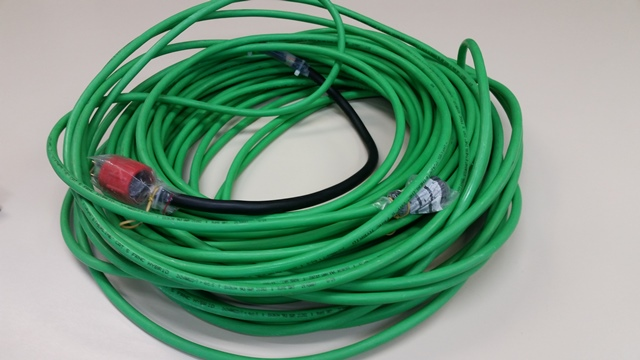
\includegraphics[width=1\columnwidth]{CaboComm/foto.jpg}
 \caption{Case da eletrônica embarcada}
\end{figure}

\subsection{Nota Fiscal}
\begin{figure}[H]
 \centering
 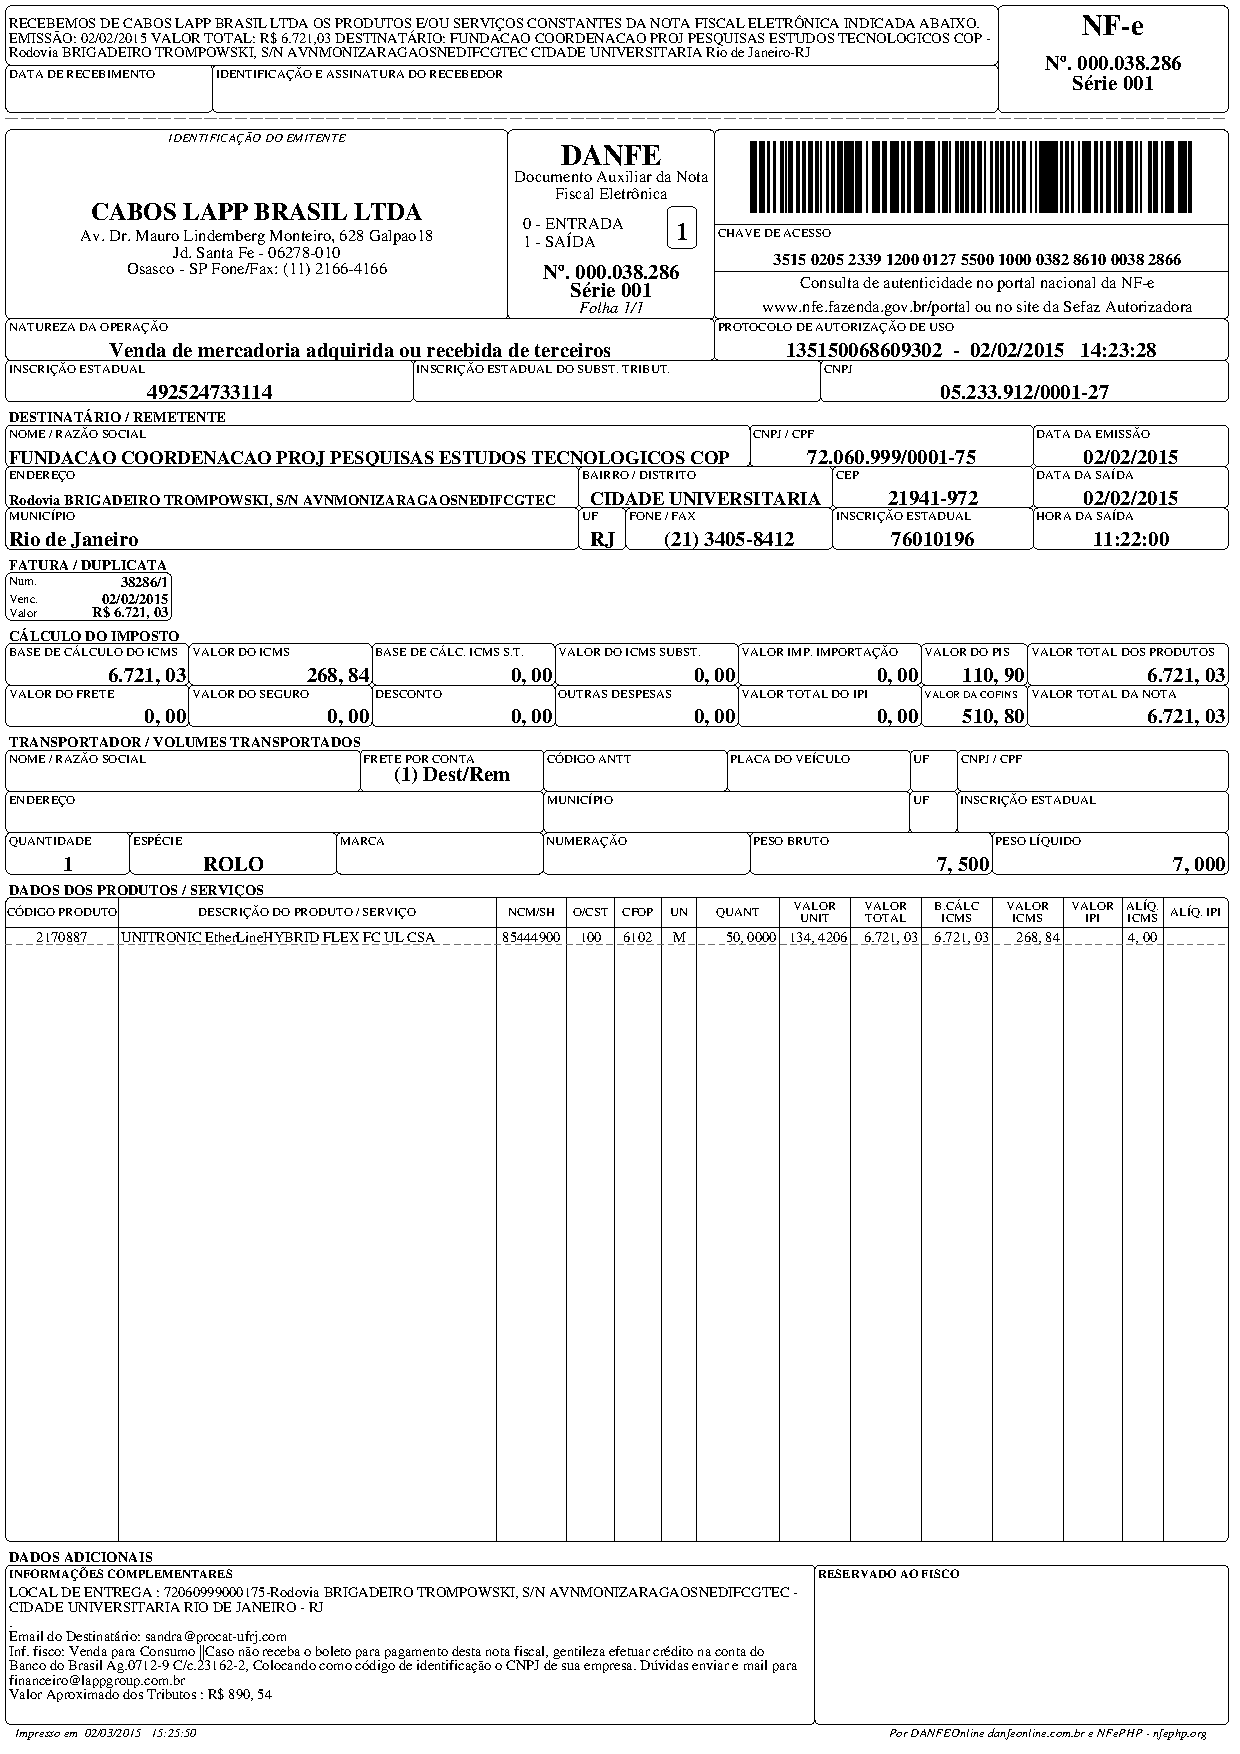
\includegraphics[width=0.9\columnwidth]{CaboComm/nota.pdf}
 \caption{Nota fiscal do Cabo de Comunicação}
 \end{figure}